\section{PLCL Material Characterization\label{methodology:materialCharacterization}}

When creating a polymer blend, characterizing the material is important to verify the material created is the desired material and composure. Material characterization can also help validate the synthesis process.

In the case of this research, externally sourced raw materials needed to be characterized to ensure their properties aligned with manufacturer data and thus behave as expected throughout the extrusion and 3D printing process.

Additionally, custom synthesized PLCL needed to be characterized to verify the composition of the blend was as expected.

\subsection{Gel Permeation Chromatography (GPC) Testing\label{sec:methodology:gpcTesting}}

Gel Permeation Chromatography (GPC) testing was conducted to evaluate the molecular weight distribution of externally sourced PLCL powder. This was done to ensure the molecular weight of the ordered powder aligned with the range provided by the manufacturer and check for any variability across batches. Molecular weight is inversely related to melt flow index which strongly impacts a material's ability to be extruded (see~\autoref{sec:literatureReview:extrusion:mechanics:parameters} for more information on melt flow index)~\cite{RefWorks:RefID:501-2024understanding}.

\subsubsection{Performing GPC Testing\label{sec:methodology:gpcTesting:performingTest}}

To perform the GPC testing, PLCL powder purchased from Nomisma was dissolved in Dimethylformamide (DMF)~\cite{RefWorks:RefID:387-nomisma}. The solution was then run through an Agilent GPC/SEC system to conduct the GPC testing.

Blank samples containing only DMF were run at the start and end to establish baselines. The testing was completed in 20 minutes. There are multiple detectors within the system, but the Reflective Index (RI) detector was utilized in this testing.

\subsubsection{Analyzing GPC Results}

A GPC test outputs a curve with various regions of interest. The curve begins and ends with a baseline region from the blank samples. The first baseline region is followed by an integration region which contains the distribution of molecular weight. The peak of the integration region corresponds to M\textsubscript{P}, the most common molecular weight of the sample. These regions are outlined below in Figure~\ref{fig:methodology:materialCharacterization:gpcCurveOverview}

\begin{figure}[H]
        \centering
        \includegraphics[width=0.5\linewidth]{../figs/methodology/materialCharacterization/gpc_curve_overview.png}
        \caption{Overview of GPC testing output curve.}
        \label{fig:methodology:materialCharacterization:gpcCurveOverview}
\end{figure}

Results and discussion of the Nomisma PLCL GPC testing can be found in~\fullref{sec:results:materialCharacterization:gpcTesting} and~\fullref{sec:discussion:materialCharacterization:gpcTesting} respectively.

\subsection{Nuclear Magnetic Resonance (NMR) Testing\label{sec:methodology:nmrTesting}}

An assessment of relevant literature illustrated that Nuclear Magnetic Resonance (NMR) testing can be utilized for determining the percent compoistion of a polymer blend (see~\fullref{sec:literatureReview:characterization:NMR}). As a result, NMR testing was researched to quantify the percent composition of extruded PLA/PCL blends. The expected composition based on the extruded blend is 70/30 PLA/PCL, but NMR testing can be used to verify the composition of the final extruded filament.

\subsection{Sample Preparation\label{sec:methodology:nmrTesting:samplePrep}}

Testing was conducted on an AVIII 400 MHz NMR machine through the department of Chemistry and Biochemistry (CBC) at The Ohio State University.

To prepare samples for NMR testing, materials were dissolved in deuterated chloroform. Because of the high sensitivity of the NMR equipment, minimal sample material was required. Single pellets of PLA, PCL, and PLA/PCL regrind were put into individual NMR tubes. This is shown in Figure~\ref{fig:methodology:materialCharacterization:nmrSamples}. The same PLA and PCL pellets that went into the PLCL extrusion were used to act as benchmarks for each material when determining percent composition (see~\autoref{sec:methodology:materialCharacterization:nmrTesting:analyzingData}).

\begin{figure}[H]
        \centering
        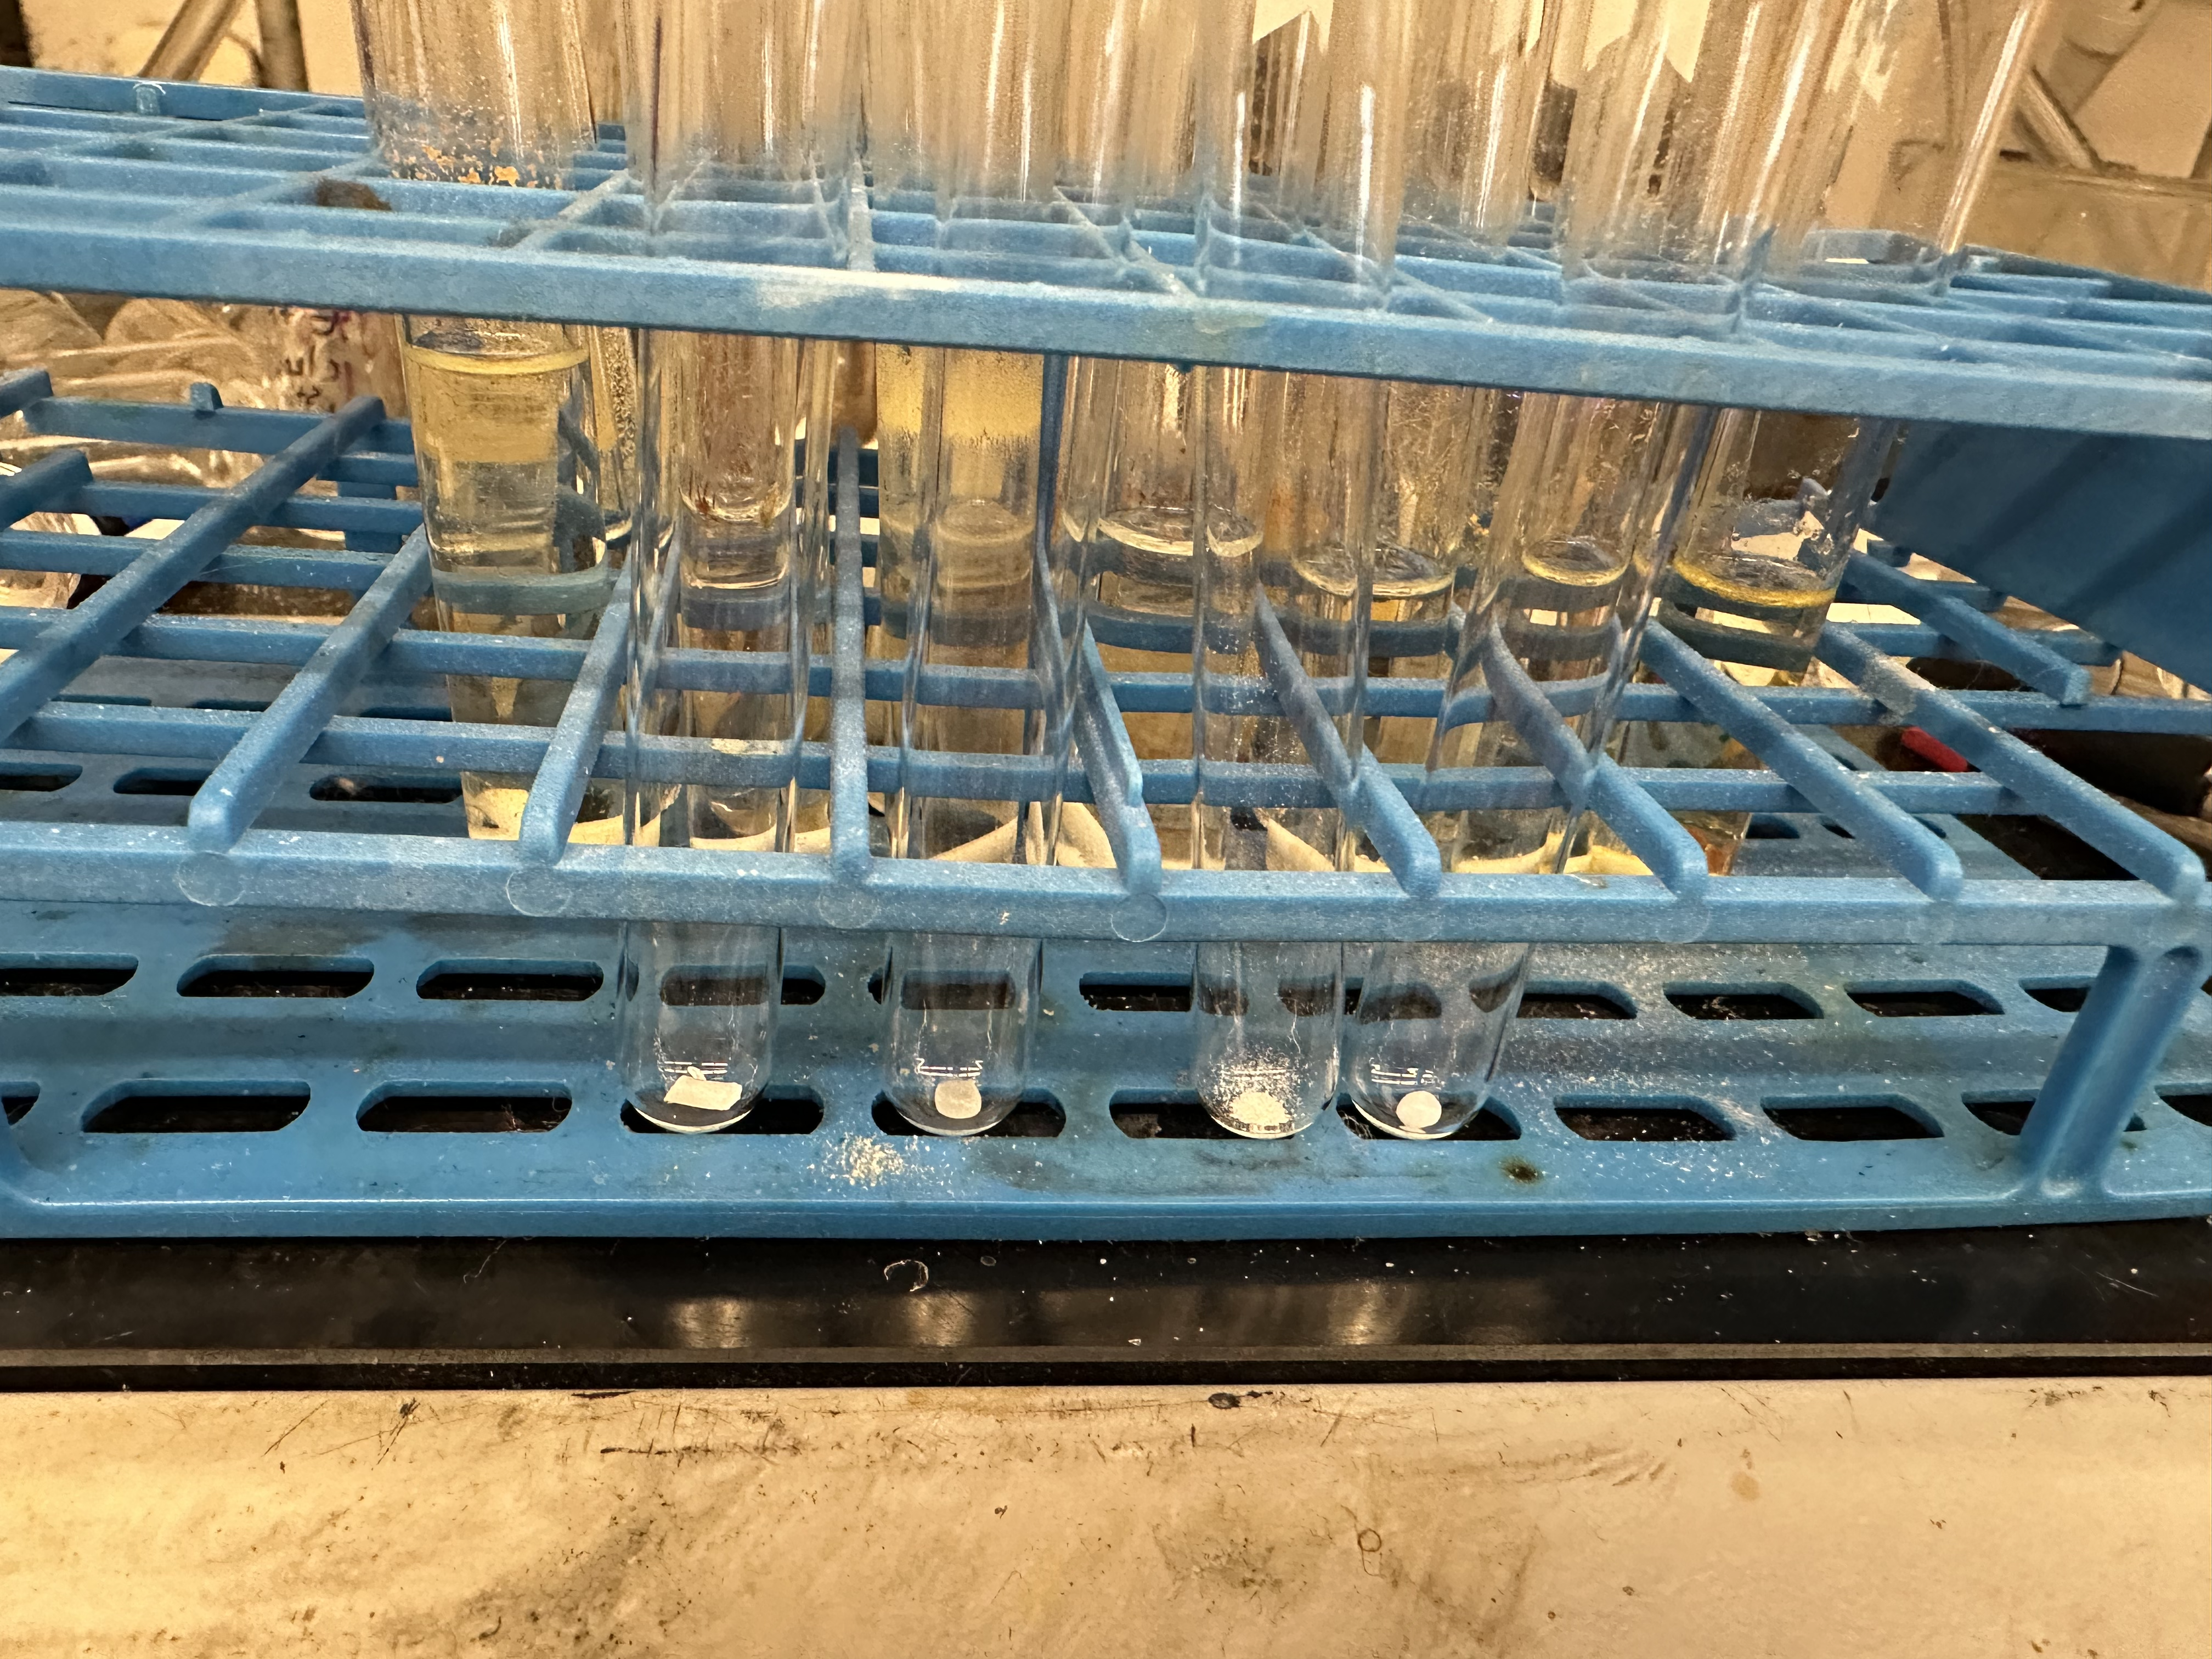
\includegraphics[width=0.5\linewidth]{../figs/methodology/materialCharacterization/nmr_sample_prep.png}
        \caption{NMR sample preparation.}
        \label{fig:methodology:materialCharacterization:nmrSamples}
\end{figure}

5$mL$ of deuterated chloroform were poured into each tube. To accelerate dissolution of material, tubes were placed in an IKA Heating Bath for five minutes as shown in Figure~\ref{fig:methodology:materialCharacterization:nmrHeatBath}.

\begin{figure}[H]
        \centering
        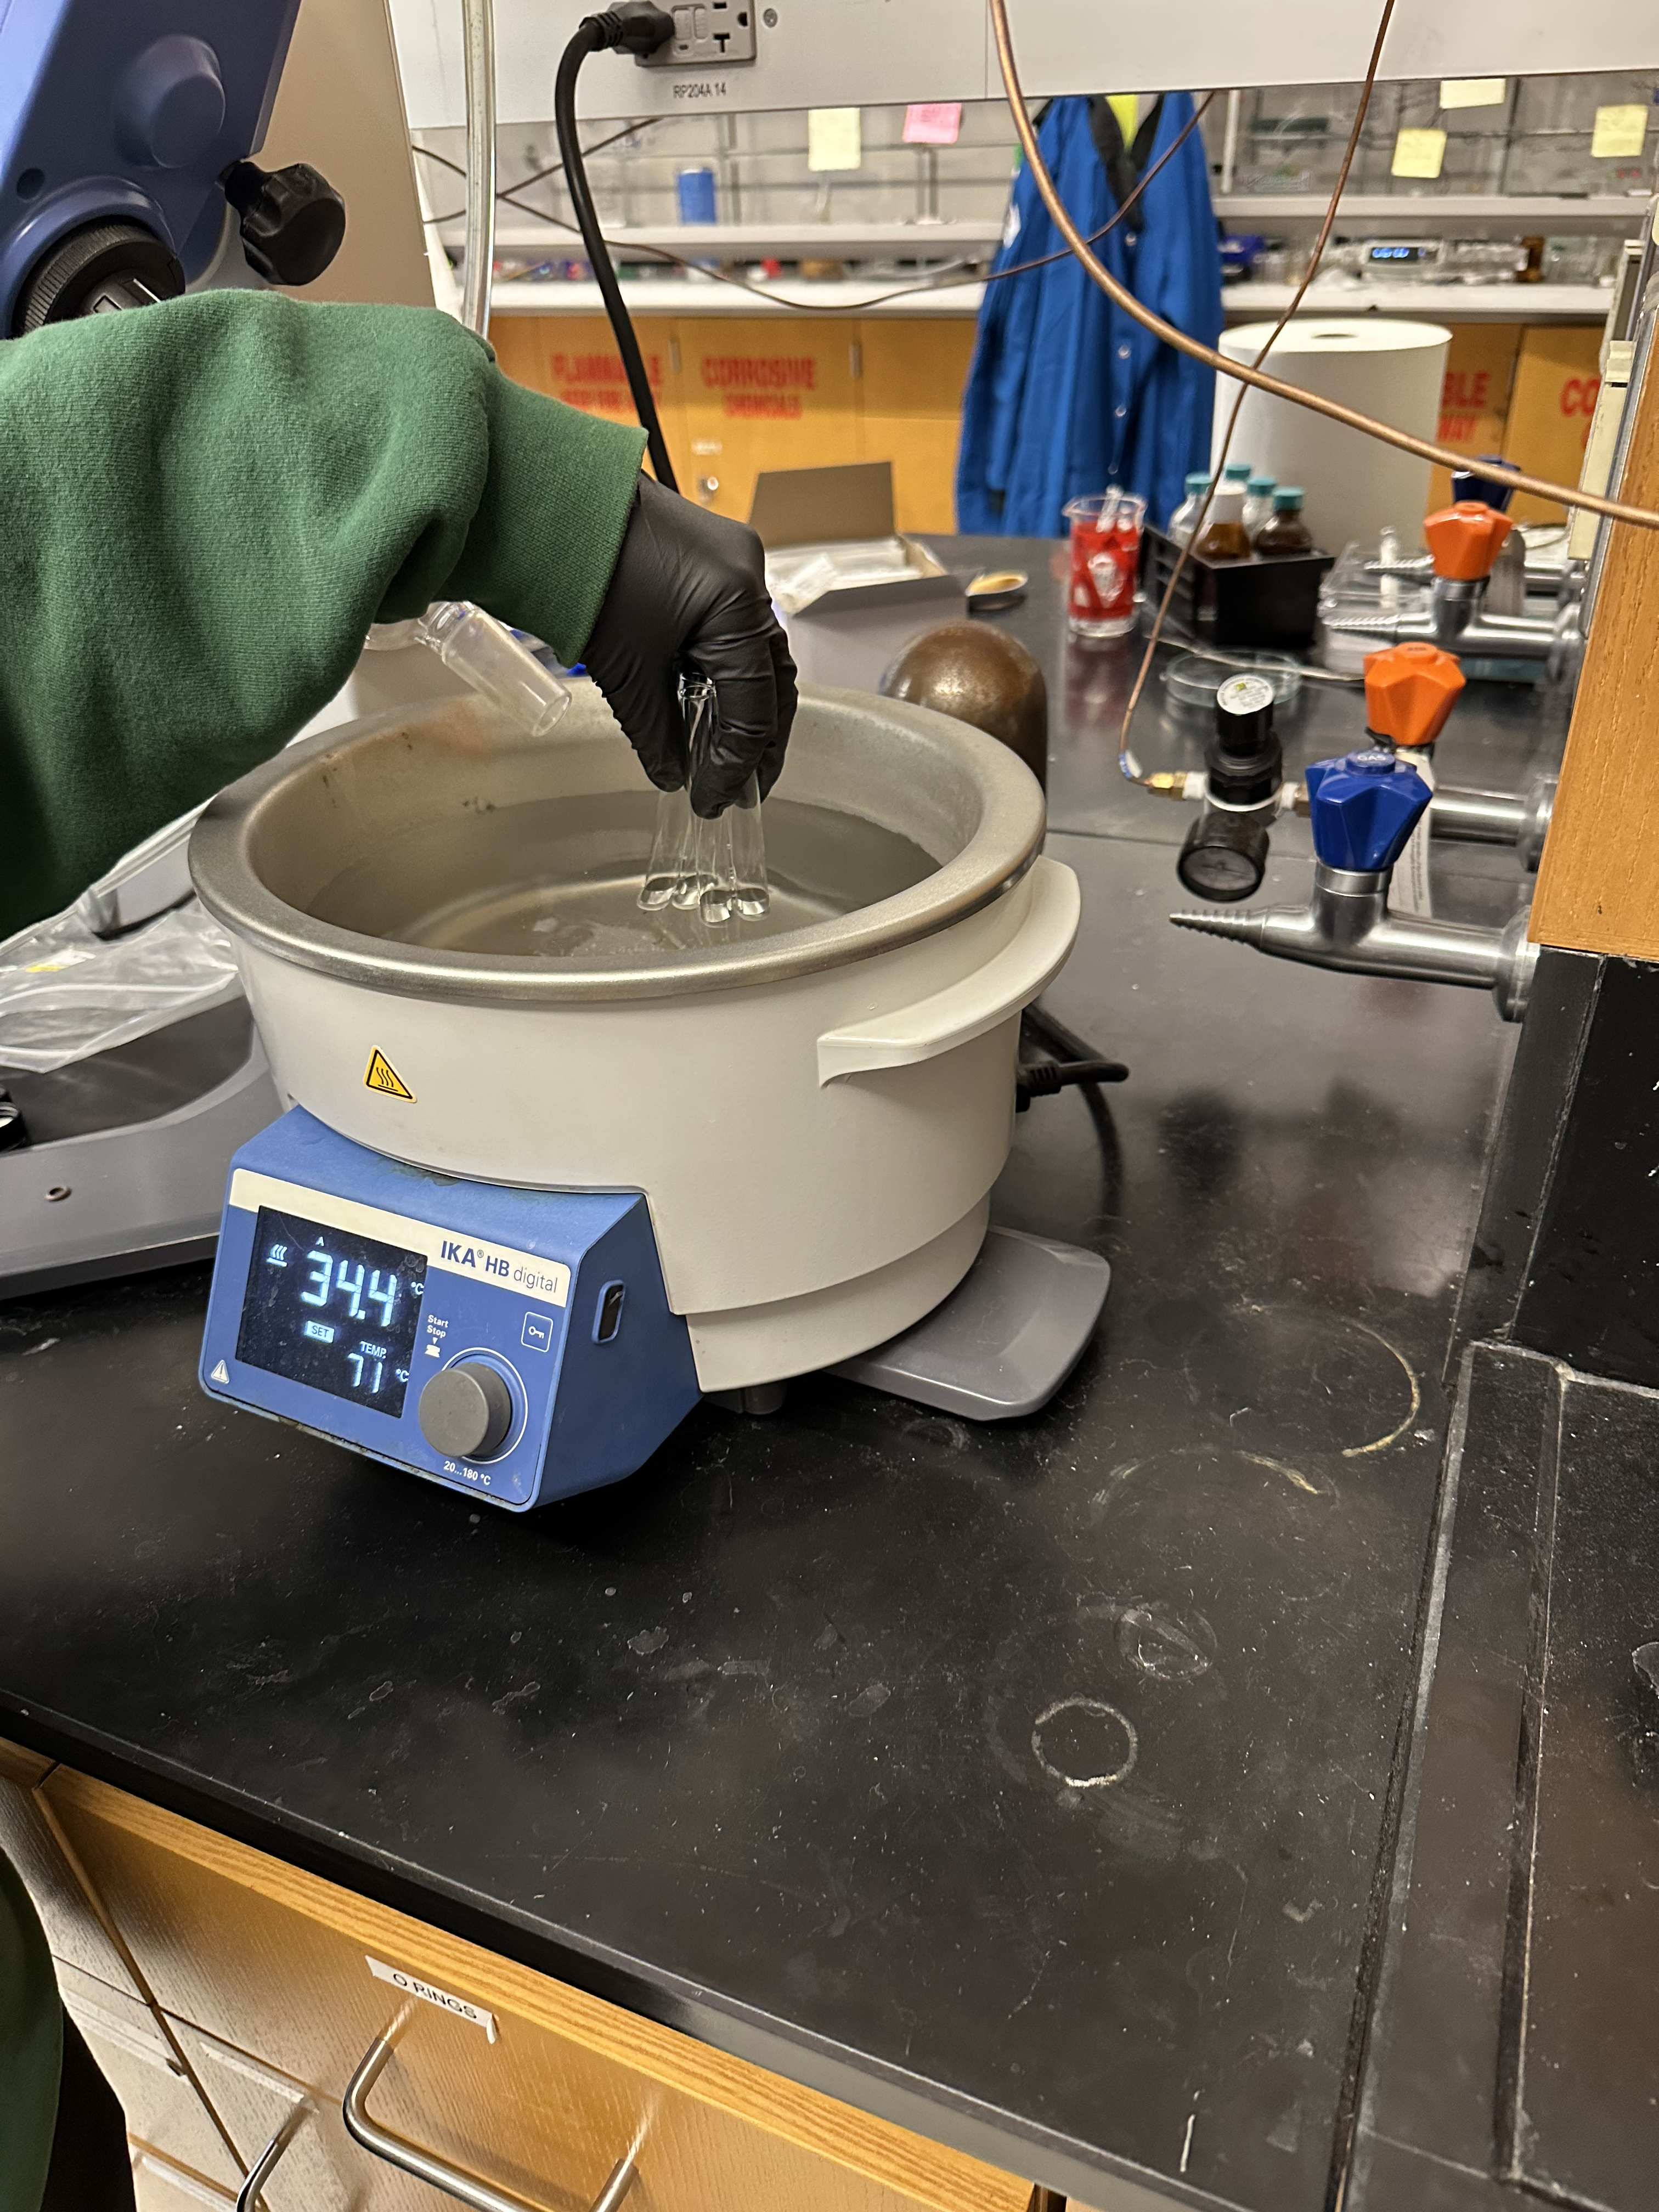
\includegraphics[width=0.5\linewidth]{../figs/methodology/materialCharacterization/nmr_heat_bath.png}
        \caption{Using a heat bath to accelerate dissolution for NMR testing.}
        \label{fig:methodology:materialCharacterization:nmrHeatBath}
\end{figure}

Once the samples were fully dissolved, the tubes were loaded into the NMR machine and set for Proton NMR.

Results and discussion of this NMR testing can be found in~\fullref{sec:results:materialCharacterization:nmrTesting} and~\fullref{sec:discussion:materialCharacterization:nmrTesting} respectively.

\subsection{Analyzing Data\label{sec:methodology:materialCharacterization:nmrTesting:analyzingData}}

To analyze the NMR spectra, a software called MestReNova was utilized as licensure was provided by The Ohio State University.

This software allows users to view and make calculations based on the NMR spectra from their testing. To calculate percent composition, peaks are first identified from each individual co-polymer spectra that were unique to that material. Then, the integral or area of that peak within the blend spectra was calculated. This integral was compared to the area of a peak from the second material within the blend spectra~\cite{RefWorks:RefID:502-schaller415}. The percent composition was then determined using Equation~\eqref{eq:nmrPercentComp}. Figure~\ref{fig:methodology:materialCharacterization:nmrPercentCompOverview}.

\begin{equation}
        Material1\% = \frac{Area_{Material1}}{Area_{Material1} + Area_{Material2}}
        \label{eq:nmrPercentComp}
\end{equation}

\begin{figure}[H]
        \centering
        \includegraphics[width=0.7\linewidth]{../figs/methodology/materialCharacterization/nmr_percent_comp_overview.png}
        \caption{Overview of calculating percent composition with NMR spectra.}\label{fig:methodology:materialCharacterization:nmrPercentCompOverview}
\end{figure}

Results and discussion of this NMR testing can be found in~\fullref{sec:results:materialCharacterization:nmrTesting} and~\fullref{sec:discussion:materialCharacterization:nmrTesting} respectively.
